% Copyright 2004 by Till Tantau <tantau@users.sourceforge.net>.
%
% In principle, this file can be redistributed and/or modified under
% the terms of the GNU Public License, version 2.
%
% However, this file is supposed to be a template to be modified
% for your own needs. For this reason, if you use this file as a
% template and not specifically distribute it as part of a another
% package/program, I grant the extra permission to freely copy and
% modify this file as you see fit and even to delete this copyright
% notice. 

\documentclass{beamer}
\usepackage[french]{babel}
\usepackage[utf8]{inputenc}
\usepackage[T1]{fontenc}
\usepackage{datetime}
\usepackage{amsmath}
\usepackage{centernot}
\usepackage{eurosym}
\setbeamertemplate{footline}[frame number]
\usepackage{graphicx}


\usetheme{Antibes}
%\usetheme{Darmstadt}
%\usetheme{Frankfurt}
%\usetheme{JuanLesPins}
%\usetheme{Madrid}
%\usetheme{Rochester}

\title{Droit du numérique}

\author{Camille Gosset\inst{1} \and Jérémie Dautheribes\inst{1}}


\institute[Universities of Somewhere and Elsewhere] % (optional, but mostly needed)
{
  \inst{1}%
    \'Etudiants en deuxième année d'informatique}
    
\date{\today}

\AtBeginSubsection[]
{
  \begin{frame}<beamer>{Sommaire}
    \tableofcontents[currentsection,currentsubsection]
  \end{frame}
}

% Let's get started
\begin{document}

\begin{frame}
  \titlepage
\end{frame}

\begin{frame}{Sommaire}
  \tableofcontents
  % You might wish to add the option [pausesections]
\end{frame}

% Section and subsections will appear in the presentation overview
% and table of contents.

\section{Protection de la vie privée}
\subsection{Vie privée}
\begin{frame}{Définition de la vie privée}
\begin{block}{Étymologie}
IV$^{ieme}$ siècle avant Jésus Christ - Aristote
\end{block}
\vspace{0.5cm}
\begin{block}{Définition}
Droit civil pour le respect des activités concernant l’intimité d’un individu
\end{block}
\end{frame}

\subsection{Droit de la vie privée}

\begin{frame}{Droit international}
  \begin{block}{Article~12 - Déclaration universelle des droits de l'Homme}
Vie privée protégée au niveau international par l'ONU
  \end{block}
\end{frame}

\begin{frame}{Droit Européen}
  \begin{block}{Article~8 - Convention européenne de la sauvegarde des droits de l'Homme}
Appartient à la vie privée tout ce qui n'a pas à être dans la sphère publique.
  \end{block}
\end{frame}

\begin{frame}{Droit Français}
  \begin{block}{Article~9 -  Code civil}
Chacun a droit au respect de sa vie privée.
  \end{block}
  \begin{block}{Article~226-1 - Répression pénale}
Est puni d'un an d'emprisonnement et de 45~000 euros d'amende le fait au moyen d'un procédé quelconque, volontairement de porter atteinte à l'intimité de la vie privée d'autrui.
  \end{block}
\end{frame}
\subsection{Protection de la vie privée en informatique}
\begin{frame}{Mentions légales}
\begin{itemize}
    \item Maîtriser les informations collectées
    \item Maîtriser qui collecte nos données
    \item Manque d'équilibre entre sécurité et protection de la vie privée
    \item Gros progrès avec la loi du \og \textsc{droit à l'oubli numérique} \fg
    \item Restriction sur la possibilité de collecter des données
    \item Conditions à accepter lors d'une première utilisation des services
\end{itemize}
\end{frame}
\begin{frame}{Blizzard Entertainement - Mentions légales}
\begin{itemize}   
\item Les conditions que nous acceptons sont définies clairement:
  \begin{itemize}
      \item Les informations collectées
      \item Ce que les entreprises vont en faire
      \item Qui rassemble, traite et utilise les informations ?
  \end{itemize}
\item Nouvelles demandes obligatoires lors d'une collecte non stipulée dans les mentions
\item Informations consultables à tout moment
\end{itemize}
\end{frame}
\subsection{Dangers et atteintes de la vie privée}
\begin{frame}
\begin{block}{PRISM}
Programme de surveillance américain - collecte de renseignements et informations personnelles
\end{block}
\begin{block}{USA PATRIOT Act}
Loi antiterroriste américaine - droit d’accès aux données 
\end{block}
\end{frame}

\section{Protection de la propriété intellectuelle}
\subsection{Propriété intellectuelle}
\begin{frame}{Définition des termes}
  \begin{block}{Définition}
    Toutes œuvres de l’esprit - propriété industrielle + propriété littéraire et artistique
  \end{block}
\begin{block}{Protection créations intellectuelles}
Obtenir des droits: INPI (Institut national de la propriété industrielle)\\
Recenser les oeuvres: OMPI (organisation mondiale de la propriété intellectuelle)
\end{block}
\end{frame}
\begin{frame}{Le libre}
  \begin{block}{Différence Libre/OpenSource}
    Libre garantit 3 libertés: liberté d’utilisation + liberté de modification + liberté de distribution \\
    OpenSource: code source ouvert
  \end{block}
  \begin{block}{Licence libre}
  Donner des droits d’auteur à une propriété intellectuelle - 4 droits fondamentaux
  \end{block}
  \begin{block}{Copyleft}
  Redistribution \Rightarrow $ Obligation de marquer la nouvelle oeuvre par un Copyleft$ ~
  
\includegraphics[scale=0.03]{Copyleft.png}
  \end{block}
\end{frame}
\subsection{Hadopi et le téléchargement illégal}
\begin{frame}{Définitions des termes}
    \begin{block}{Le téléchargement illégal} 
    \begin{itemize}
        \item Consiste à acquérir des œuvres protégées (film, musique, jeux, etc.) par la propriété intellectuelle (droits d'auteurs) sans rémunérer d'une quelconque façon les auteurs et producteurs.
        % Estimation de 13 millions de françaos sur un site de téléchargement illégal au moins une fois par mois?
        \item En 2013, on estime que 13 millions de français sont allés sur un site de téléchargement illégal au moins une fois par mois
    \end{itemize}
   \end{block}
   \begin{alertblock}{Remarque}
    Droit à la copie privée: pouvoir copier à des fins privées des oeuvres acquises légalement
   \end{alertblock}
    
\end{frame}
\begin{frame}{Hadopi}
  Création de la : \\
  \centerline{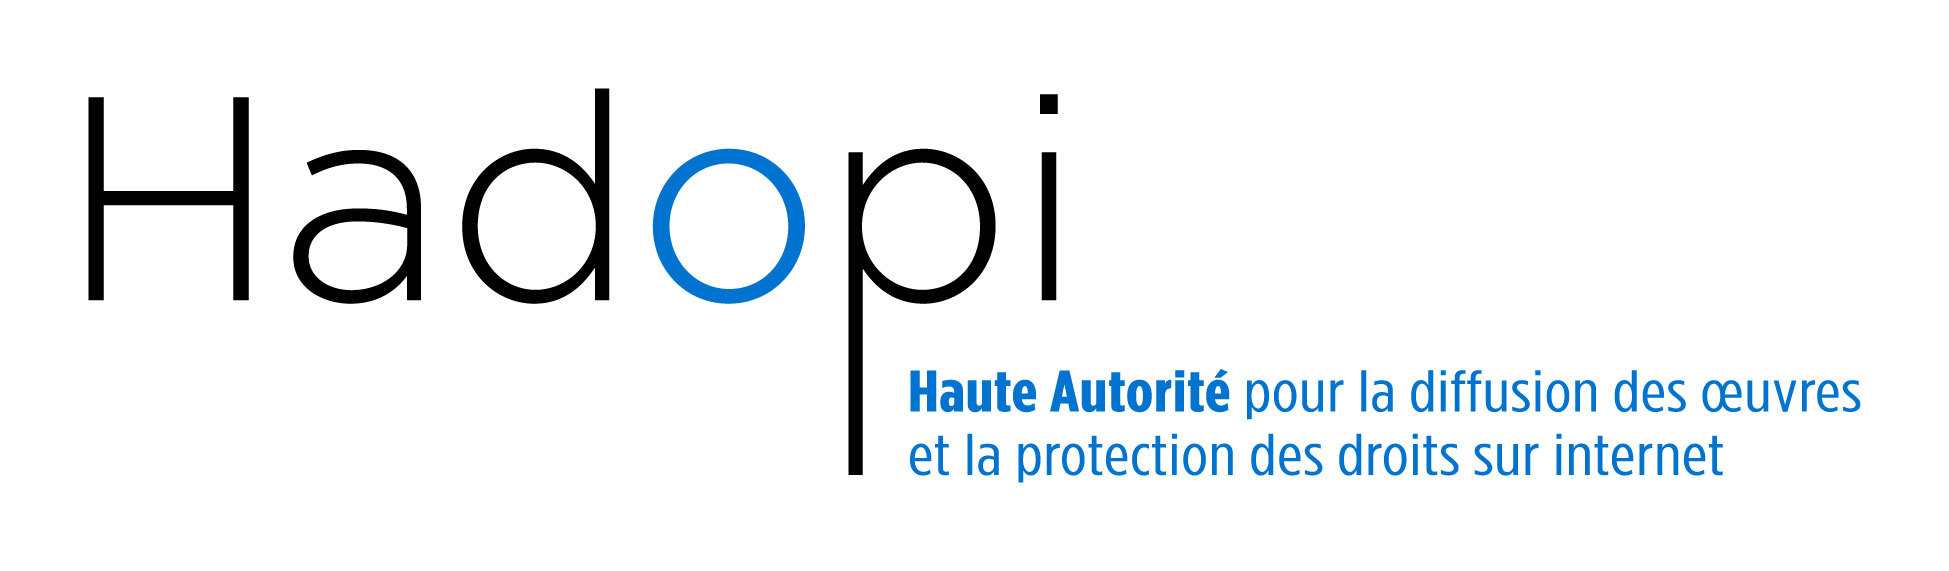
\includegraphics[scale=0.4]{hadopi.jpg}}
  \\ % Super slide
  \begin{block}{Si la Hadopi détecte une adresse IP récurrente :}
  \begin{itemize}
      \item Un premier mail est envoyé (rappel à l'ordre)
      \item Un deuxième mail est envoyé si l'adresse IP est détectée dans les 6 mois suivants l'envoie du premier mail
      \item Si dans les 12 mois suivants l'envoie du premier mail l'adresse IP est détectée une troisième fois, risque pénal (jusqu'à 1500\euro ~d'amende)
  \end{itemize}
  \end{block}
  
\end{frame} 
% Très bien
\begin{frame}{Vers la fin de la Hadopi ?}
\begin{block}{Des signes inquiétants}
    \begin{itemize}
        \item Vivement constestée à sa création et encore plus aujourd'hui
        \item Réduction du budget (11M \euro ~en 2011, 5.4M \euro ~aujourd'hui)
        \item Fermeture anciennement prévue pour 2022 avant d'être finalement annulée
    \end{itemize}
\end{block}

    \begin{block}{Une vague de changements}
    % Eloignement de la répression .. et direction vers une mise en avant ... ? 
    Éloignement vis à vis de la répression (sans pour autant l'abandonner) et direction tournée vers une mise en avant des offres légales
    \end{block}
  
\end{frame}

\section{Accessibilité numérique contre la fracture numérique}
\subsection{Définition}
\begin{frame}{Définition}
    \begin{block}{La fracture numérique}
        \begin{itemize}
            \item Ensemble des disparités d'accès aux technologies informatiques, dont notamment internet
            \item À toutes les échelles : mondiale, nationale, régionale
            \item Géographique et sociale
            \item Marquée entre les pays riches et les pays pauvres, et entre les métropoles et les zones peu denses et rurales
        \end{itemize}
    
    \end{block}
    \begin{alertblock}{Remarque}
    Droit d'accès à internet: de plus en plus reconnu en France et en Europe
    
    \end{alertblock}
  
\end{frame}

\subsection{Dans le monde}
\begin{frame}{Accès à internet}
    \centerline{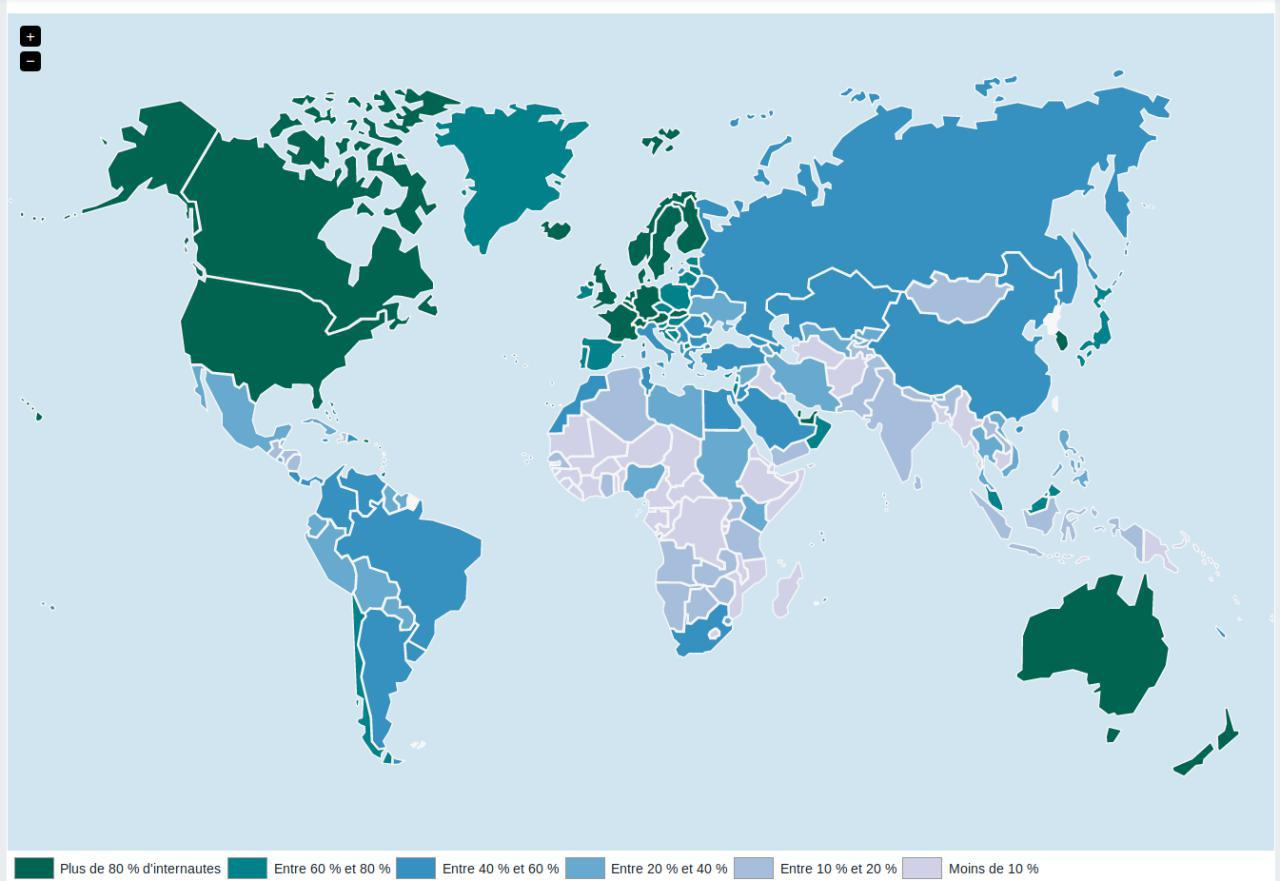
\includegraphics[scale=0.475]{acces_internet_mondial.jpg}}
    \centerline{Carte du taux d'accès à internet dans le monde, 2012.}
\end{frame}

\begin{frame}{Solutions et projets}

\begin{figure}
    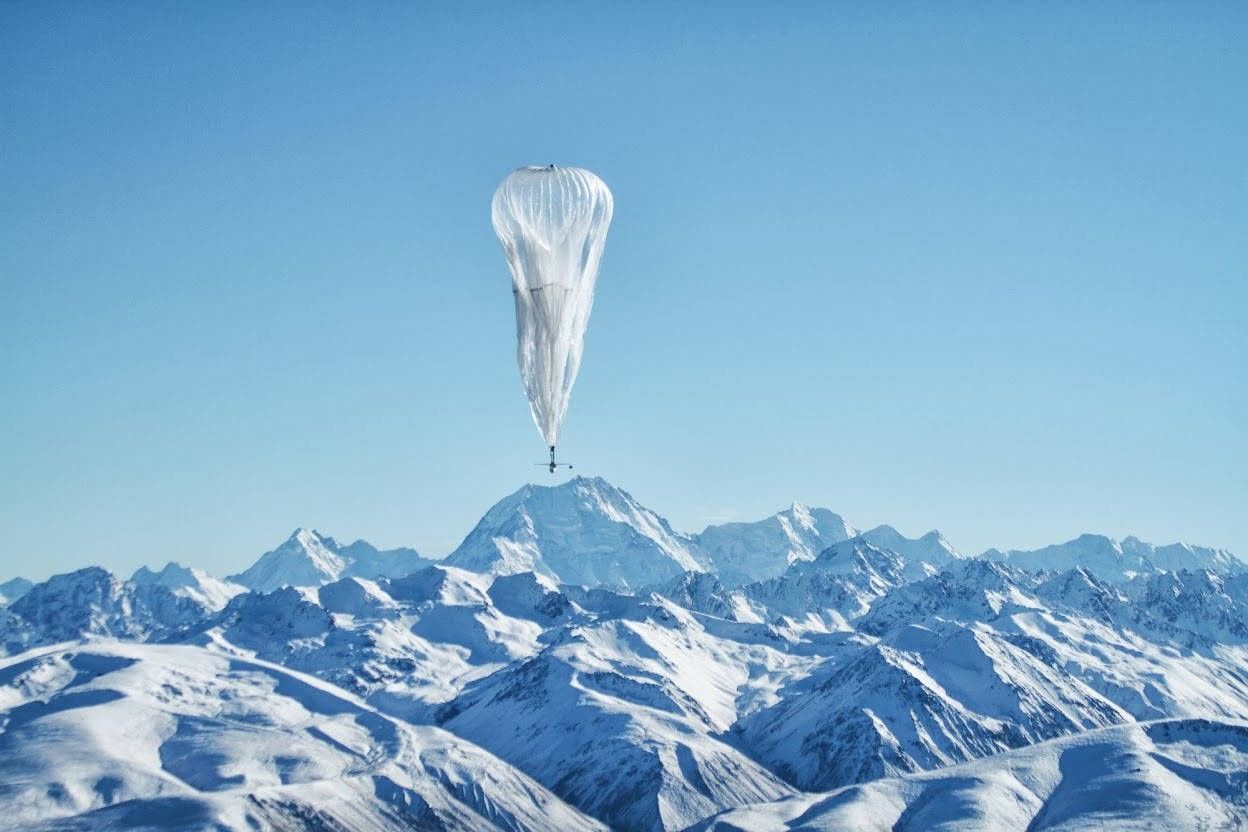
\includegraphics[width=0.475\textwidth]{loon.jpg}
    \hfill
    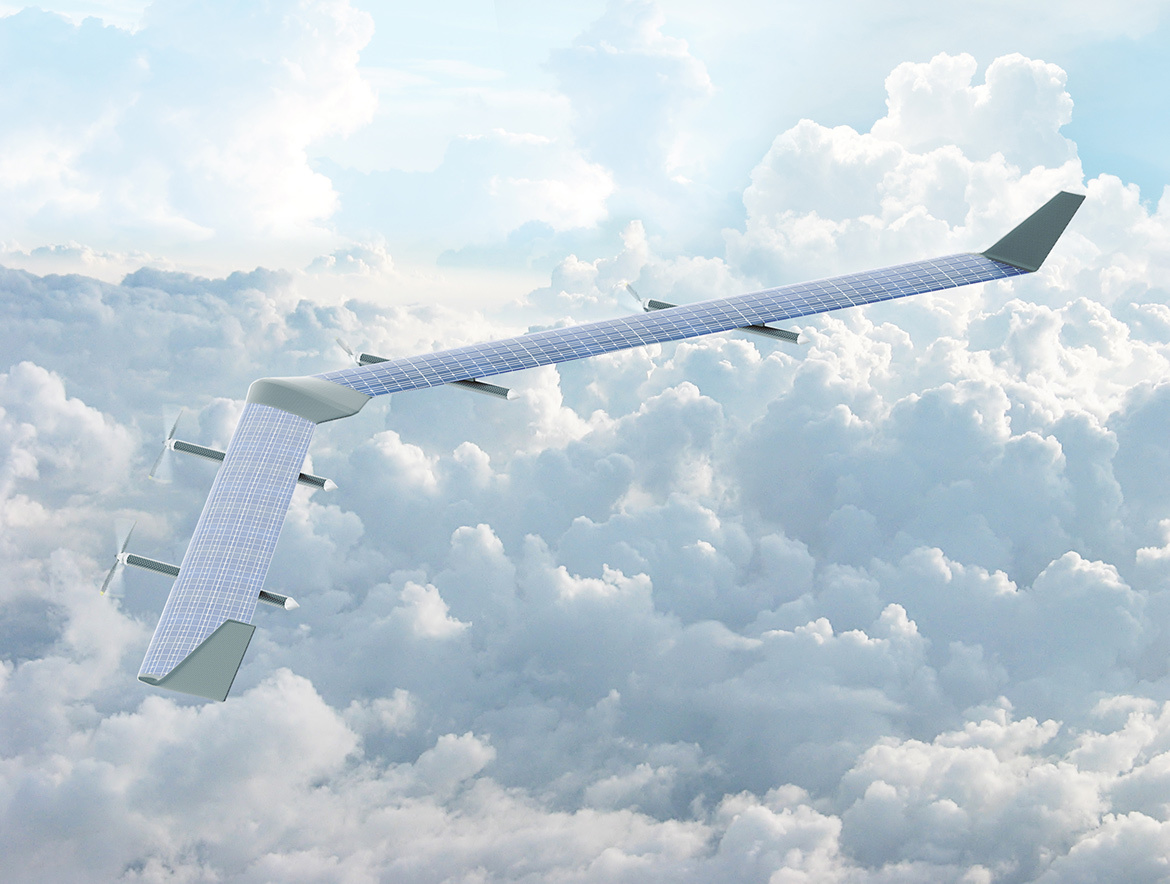
\includegraphics[width=0.475\textwidth]{aquilla.jpg}
    \caption{Respectivement , projets Loon de Google et Aquilla de Facebook}
\end{figure}


  
        
   
            
  
            
        
  
\end{frame}


\subsection{En France}
\begin{frame}{Réseau mobile}
  \centerline{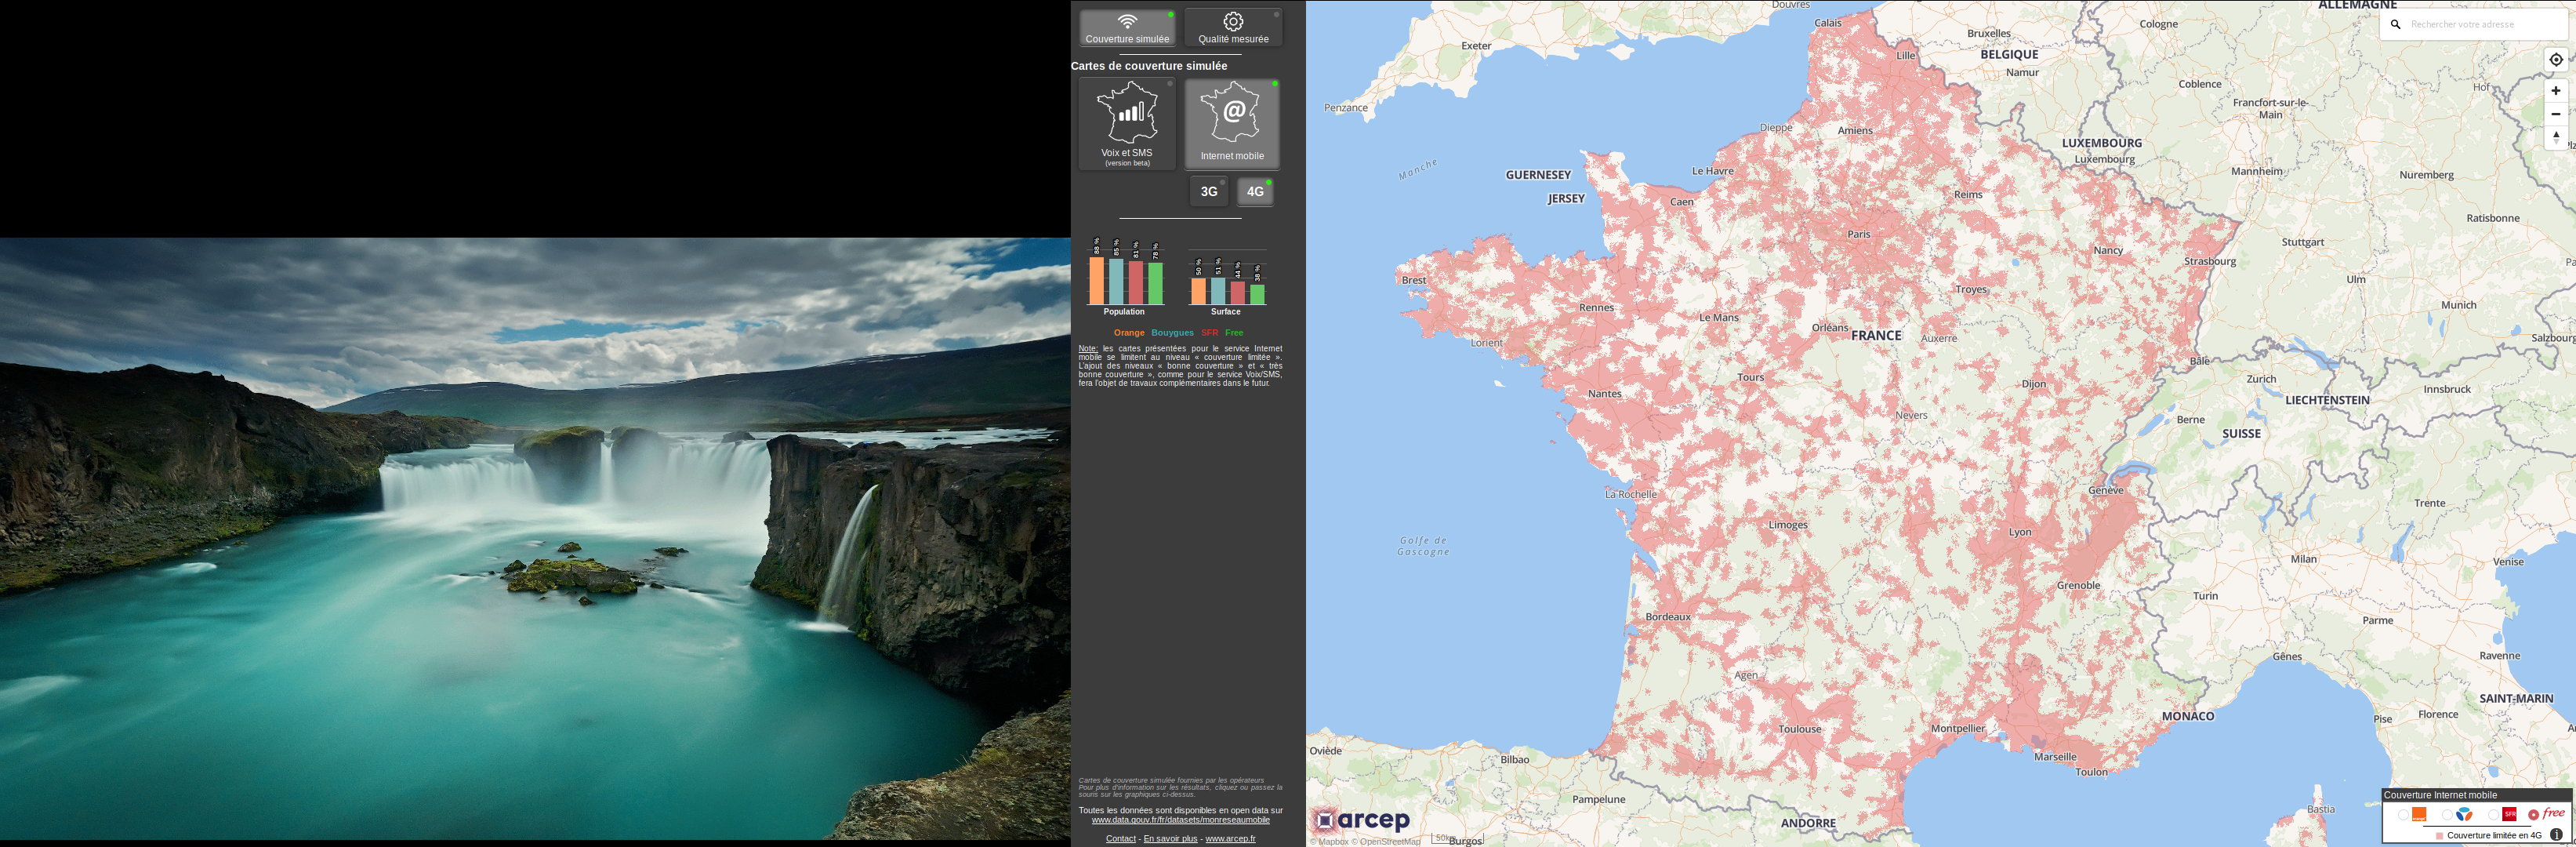
\includegraphics[trim = 60cm 0cm 15cm 0cm, clip=true ,scale= 0.16]{4g.png}}
  \centerline{Déploiement du réseau 4G en France - Hiver 2017}
\end{frame}

\begin{frame}{Arcep - I}
\begin{block}{Autorité de régulation des communications électroniques et des postes}
Les objectifs sont fixés sur : 
\begin{itemize}
    \item Le pourcentage de couverture de la population
    \item Le pourcentage de couverture du territoire
    \item Le déploiement des différentes technologies mobiles : 2G, 3G, 4G et bientôt 5G
    \item La couverture de certains territoires particuliers: les zones blanches, les axes routiers et ferroviaires, ...
\end{itemize}
\end{block}
\end{frame}

\begin{frame}{Arcep - II}
\begin{block}{Quelques objectifs:}
\begin{itemize}
    \item 100\% des zones blanches en 2G fin 2016, en 3G mi-2017 et en 4G en 2027
    \item 100\% des zones peu denses en 4G en 2022
    \item 60\% du réseau ferroviaire en 4G en 2022
\end{itemize}
\end{block}
    
\end{frame}

\begin{frame}{Déploiement de la fibre}
    \centerline{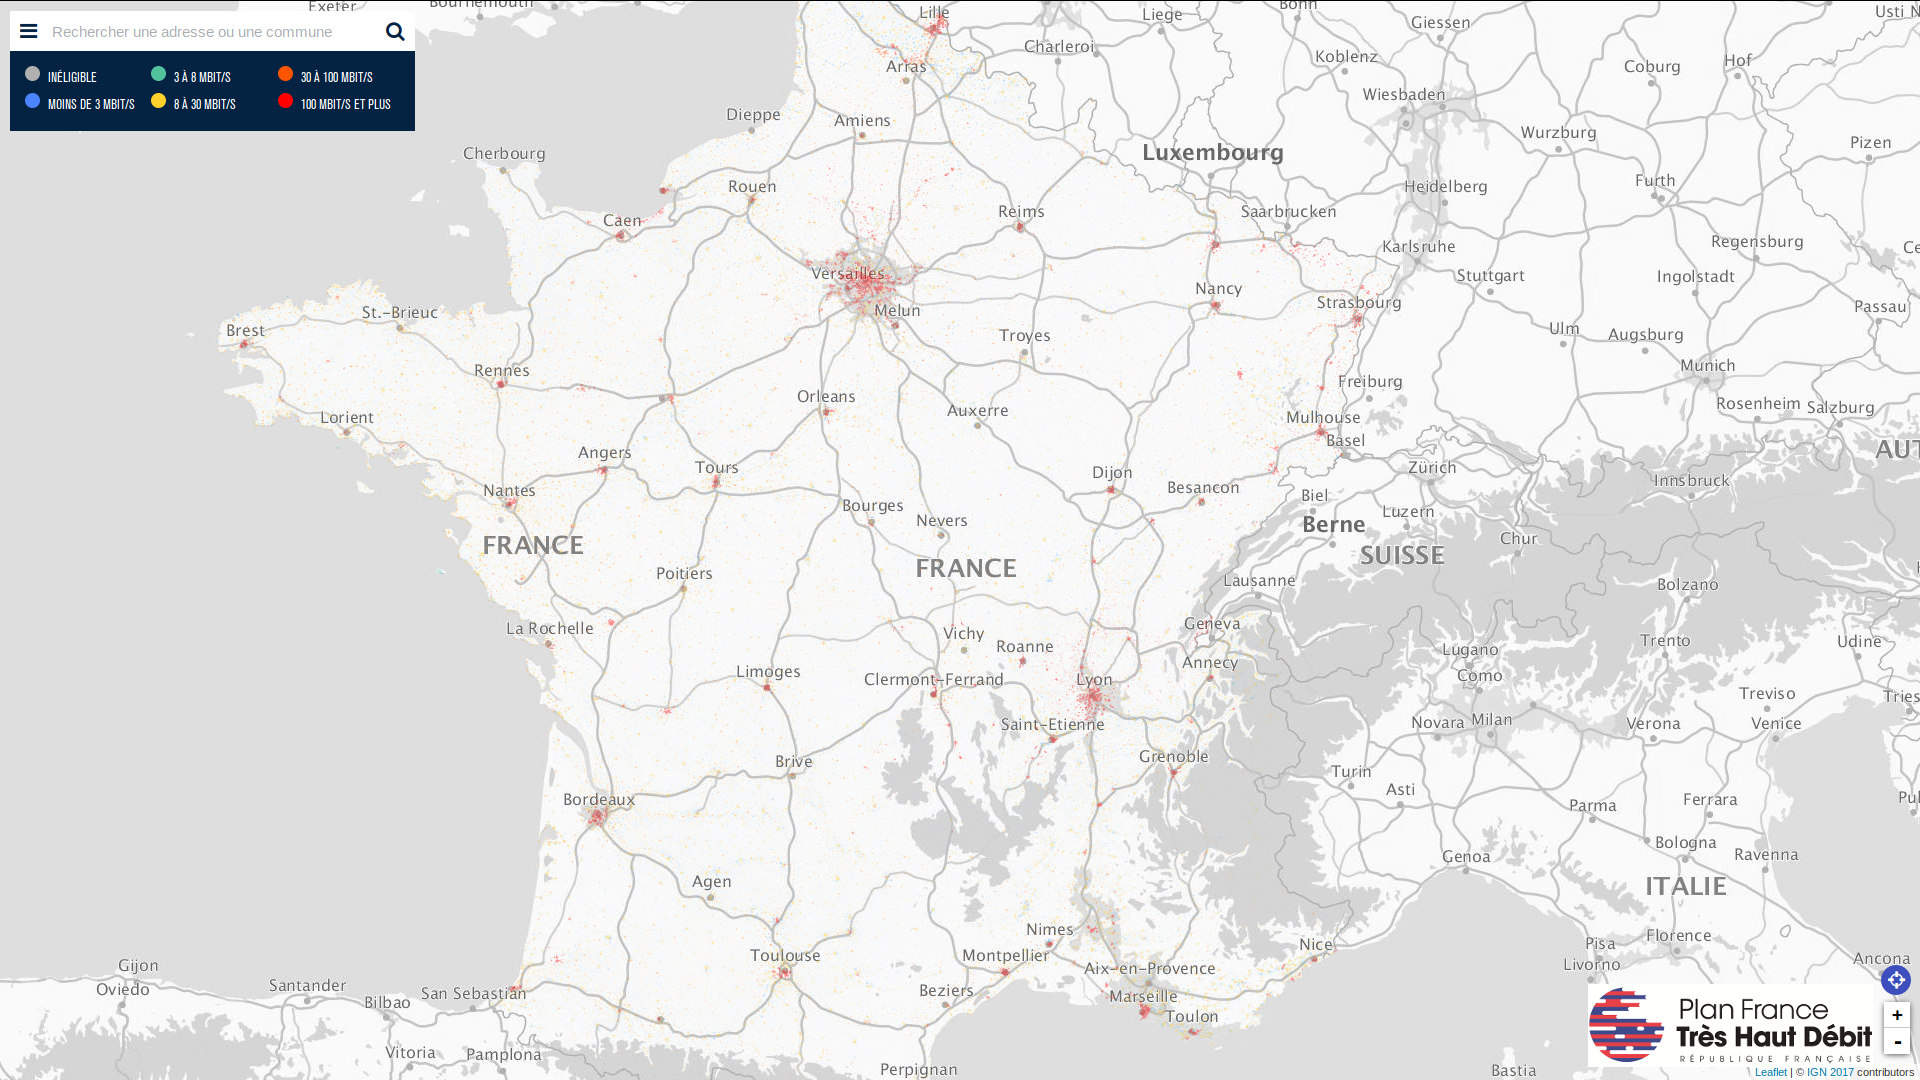
\includegraphics[trim = 0cm 0cm 15cm 0cm, clip=true, scale=0.15]{fibre.png}}
    \centerline{Déploiement de la fibre - Mai 2017}
\end{frame}

\begin{frame}{Plan Très Haut Débit (THD)}
    \begin{block}{Plan THD}
    \begin{itemize}
         \item Lancé en 2013
         \item 100\% de la population connectée au très haut débit d'ici 2022
    \end{itemize}
    \end{block}
    \begin{alertblock}{Remarque}
        Le très haut débit correspond à un débit descendant \geq 30Mbit/s
    \end{alertblock}
\end{frame}
\section*{Conclusion}

\begin{frame}{Conclusion}
  \begin{itemize}
  \item
    La \alert{protection de la vie privée } en informatique: droit permettant de gérer le type d'informations collectées et par qui, de savoir quelles informations sont collectées sur nous et ce qui en est fait.
  \item
    La \alert{protection de la propriété intellectuelle}: droit pour protéger l'auteur victime d'un plagiat ou d'une contrefaçon.
  \item
    L'\alert{accessibilité numérique contre la fracture numérique} est appuyée par le droit d'accès à internet pour réduire la fracture numérique.
  \end{itemize}
  
  \begin{itemize}
  \item
    Ouverture:
    \begin{itemize}
    \item
      Jusqu'à quel point pouvons nous accepter que le numérique empiète sur notre vie privée?
    \end{itemize}
  \end{itemize}
\end{frame}



% BIBLIO 
\appendix
\section<presentation>*{\appendixname}
\subsection<presentation>*{Bibliographie}

\begin{frame}[allowframebreaks]
  \frametitle<presentation>{Bibliographie}
    
  \begin{thebibliography}{10}
  \beamertemplatebookbibitems
  \bibitem{droit}
  \href{https://www.legifrance.gouv.fr}{Legifrance }
  
  \beamertemplatebookbibitems
  \bibitem{droit2}
  \href{http://www.dalloz-actualite.fr}{Dalloz actualité}
  
  \beamertemplatearticlebibitems

  \bibitem{Engagement sur la confidentialite}
    Blizzard
    \newblock \href{http://eu.blizzard.com/fr-fr/company/about/privacy.html}{Engagement sur la confidentialité}
    
    \beamertemplatearticlebibitems
\bibitem{Textes officiels CNIL}
    CNIL
    \newblock \href{https://www.cnil.fr/fr/textes-officiels-europeens-protection-donnees}{Textes officiels européens sur la protection des données}
    \\ \href{https://www.cnil.fr/fr/comprendre-le-reglement-europeen}{Comprendre le règlement européen}
    
    \beamertemplatearticlebibitems
    \bibitem{site de l'INPI}
    \href{https://www.inpi.fr/fr}{INPI}
    \newblock site officiel de l'INPI
  \end{thebibliography}
\end{frame}

\end{document}


